\documentclass[12pt,a4paper]{article}
\usepackage{times}
\usepackage{durhampaper}
\usepackage{harvard}
\usepackage{underscore}
\usepackage{graphicx}
\usepackage{caption}
\usepackage{subcaption}
\usepackage{url}
\usepackage{hyperref}
\usepackage[subtle]{savetrees}
\usepackage[ruled,vlined,linesnumbered]{algorithm2e}


\citationmode{abbr}
\bibliographystyle{agsm}

\title{Procedural World Building in Roguelike Games}
\author{Benjamin Jones}
\student{Benjamin Jones}
\supervisor{Dr Tom Friedetzky}
\degree{MSci Natural Sciences}

\date{}

\begin{document}

\maketitle

\begin{abstract}

{\bf Context/Background}

Procedural content generation in videogames has seen a surge in popularity in recent years. However as game development progress, users expect more and more intelligent and engaging game level design and as a result, investigating new, interesting methods of procedural content generation is vital to keeping end users happy.

{\bf Aims}

This project aims to draw comparisons between current methods of procedural content generation in a roguelike game environment and build upon them to create different and exciting methods of level design. The implementation will focus on creating a number of novel algorithms alongside an intelligent method of evaluating their suitability. 

{\bf Method}

A variety of algorithms will be developed and implemented by building on and combining various existing methods found in existing roguelikes and more sophisticated modern games. Perlin and Simplex noise algorithms will be used to generate the initial random seed, which will then be modified by a variety of methods including the \emph{Cellular Automata} approach and the use of geometric space-filling curves such as the Hilbert curve and Sierpinski curve. The effectiveness of these will then be evaluated by a custom heuristic, ensuring the quality of the resulting world. 

% {\bf Proposed Solution}

% The proposed game will be built and played in Java using the \emph{JFrame} and \emph{asciipanel} libraries as a framework. The combination of existing algorithms and novel techniques will produce multiple potential procedurally generated worlds, which will be evaluated by the program and the best fit will form the playable environment in a roguelike game. 

{\bf Results}

{\bf Conclusion}

\end{abstract}

% \begin{abstract}
% These instructions give you guidelines for preparing the final paper.  DO NOT change any settings, such as margins and font sizes.  Just use this as a template and modify the contents into your final paper.  Do not cite references in the abstract.

% The abstract must be a Structured Abstract with the headings {\bf Context/Background}, {\bf Aims}, {\bf Method}, {\bf Results}, and {\bf Conclusions}.  This section should not be longer than half of a page, and having no more than one or two sentences under each heading is advised.
% \end{abstract}

\begin{keywords}
Procedural content generation, roguelike, world building, noise algorithms, artificial intelligence, heuristic, space-filling algorithms.
\end{keywords}

\section{Introduction}


\subsection{Roguelike Games}

The term Roguelike [CAPITALISE OR NOT? emph?] stems from the original 1980s UNIX dungeon crawler \emph{Rogue} created by Michael Toy and Glenn Wichman, giving birth to hundreds of games such as \emph{Nethack} and \emph{Dwarf Fortress} that follow the same style and structure and revolutionising the gaming industry as we know it today \cite{Dunhack}. There are many different styles of roguelikes these days, but most share the same core features: turn-based gameplay, procedurally generated tile-based dungeons or maps, and randomly created monsters and items \cite{pgcbook}. \\


The basic premise of the game has the player controlling a single character through numerous ASCII represented areas filled with monsters, items and traps. However what made it so revolutionary at the time was the fact that the game was different (and the gameplay unique), every time you played it thanks to its procedurally generated nature, and its ability to create an infinite set of playable dungeons was unparalleled\cite{platformgames}. However these days players expect more from games and this work aims to advance on the relatively primitive types of procedural generation seen in these early fan favourites. \\


This work aims to investigate existing methods of procedural generation within videogames and create a new approach that is both visually appealing and interesting to play to meet the increasing demands of the modern gamer. The genre of roguelike games provides an excellent [appropriate?] framework for this aim, combining sufficient complexity with an appropriate method of visualisation of the algorithms. [not sure about this?]

% other types of roguelike can be discussed in the previous work area

% Diablo, spore

\subsection{Procedural Content Generation}

Procedural content generation (PCG) is the process of creating content through the use of random numbers as seeds to generate objects using algorithms and mathematical functions, as opposed to the typical method of being manually created by a developer \cite{pgcbook}. This has many possible applications, from running real-world simulations on procedurally generated objects and environments \cite{VAST}, to generating interesting and unique textures and graphics \cite{imagesynth}, and of course for use in video games. In short, this is typically achieved by modifying the results of mathematical noise algorithms \cite{pgcbookch4}, which generate heightmaps or intensity maps that can be adapted to create procedurally generated content, such as terrains or graphics \cite{improvepnoise}.  \\


Procedural generation has many advantages unrivalled by other generation methods: it is typically much faster to evaluate, it has the ability to generate arbitrarily complex and intricate designs on-the-fly and has a particularly low memory footprint \cite{surveyPNF}. Additionally, the variation of input parameters can easily generate an incredible number of uniquely styled designs. The result is that procedurally generated game content has the capability to offer every game user a unique gaming experience every time they play. \\

% One of the most advanced examples of PCG in roguelikes to date is Bay12Games's 2006 creation Dwarf Fortress. 

A perfect example of the power and potential of PCG is \emph{Minecraft}. At the time of writing, \emph{Minecraft} sales have hit more than 70 million world-wide, making it one of the most popular games of all time \cite{ukie}. However at it's base, \emph{Minecraft} draws many parallels with the methods of generation seen in even some of the earliest Roguelike games, for example it uses at its core a 3D adoption of the 2D Perlin fractal noise algorithm adopted by many popular Roguelikes \cite{notch}, including the 2006 variant, \emph{Dwarf Fortress} \cite{Dunhack}. \\


Also recently hitting the spotlights recently is indie game \emph{No Man's Sky}, a futuristic sci-fi role-playing game (RPG) that procedurally generates an entire universe populated with up to 18 quintillion planets for the player to explore at their leisure \cite{E3} [IS THIS HOW TO CITE A CONFERENCE?]. Developed by a team of only 10 people, \emph{No Man's Sky} demonstrates the power and potential that procedural generation has to offer to the gaming market. \\


A final game worth mentioning is award-winning 2004 German 3D shooter \emph{.kkrieger}. The game won its award not because of its content however, but because of its extensive use of procedural generation techniques mean everything from the textures to the in-game sounds (as well as the traditional monsters and levels) are generated completely procedurally. This allows the entire game to be coded in just 96 kilobytes of memory, meaning that even screenshots of the game take up more room than the game itself- allowing \emph{.kkrieger} to take up 3000x less storage than an equivalent conventionally designed game \cite{kkrieger}. This game exemplifies what can be achieved using procedural techniques. \\

As games get more complex and take longer to build, coming up with new and exciting ways to programatically generate game content could be the key to a revolution a game industry expected to reach \$103bn in 2017 \cite{newzoo}. Furthermore, as the industry continues to get more and more competitive, procedural generation is likely to play a key role in allowing indie game developers to keep up with their big-budget counterparts.

\subsection{Contribution Direction}

While roguelikes and their derivatives remain popular more than 40 years after their introduction, current favourites such as \emph{Nethack} and \emph{Dwarf Fortress} struggle to bridge the gap between being visually appealing and functionally engaging. While \emph{Nethack} offers intricate and complex gameplay mechanics, its level design is basic and while more recent editions have offered a graphical tile-based experience, it fails to keep up with the demands of the modern market. On the other hand, \emph{Dwarf Fortress} offers incredibly complex algorithmic techniques (owing to its 10 years of open source development), but again falls short in level aesthetics. \\

This work aims to bridge the gap filled by a generation of roguelikes, intending to create worlds in a roguelike setting that are both visually pleasing to the modern gamer whilst maintaining the complexity and gameplay aspects that have enticed thousands of players over the years. We predicted that successful implementations of procedural content generation, both in roguelikes and in a wider context, have the ability to satisfy gamers while reducing the cost of content creation significantly, as well as increasing entertainment and replayablility. The latter not only has important implications in the well established single-player market, but also in the expansive domain of massively multiplayer online games (MMOGs), most of which gain revenue from the continued and repeated involvement of players month to month, and estimated to lead the global games market in 2018 with a predicted revenue of approximately \$34.3bn dollars \cite{newzoo}. 

\begin{figure}
\centering
\begin{subfigure}{.5\textwidth}
  \centering
  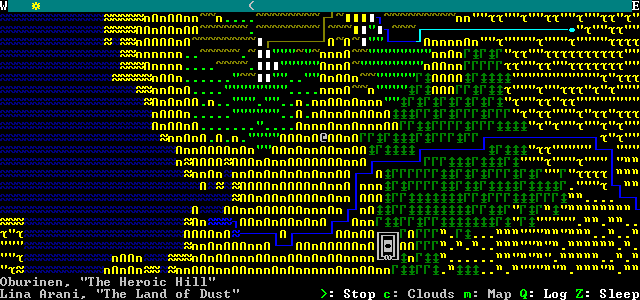
\includegraphics[width=.6\linewidth, height=3cm]{images/dwarffortress.png}
  \caption{A sample of the playable overworld in \emph{Dwarf Fortress}. Image sourced from: http://www.bay12games.com}
  \label{fig:sub1}
\end{subfigure}%
\begin{subfigure}{.5\textwidth}
  \centering
  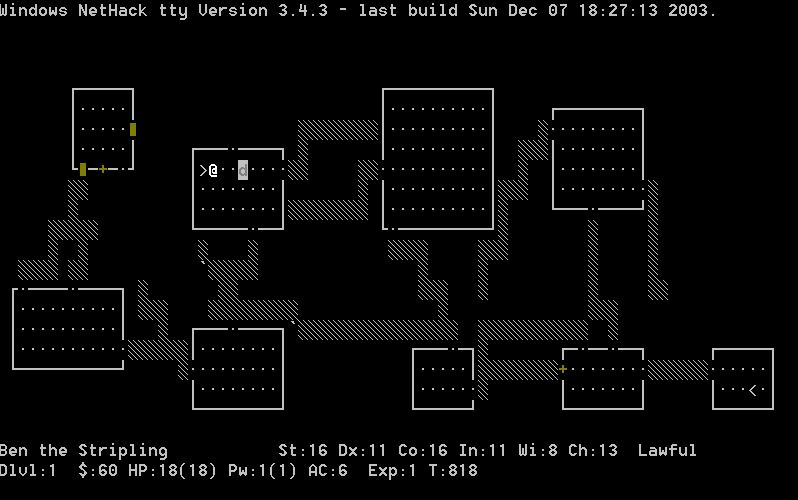
\includegraphics[width=.6\linewidth, height=3cm]{images/nethack3.png}
  \caption{Typical generated dungeon structure in \emph{Nethack}.}
  \label{fig:sub2}
  \ \\
\end{subfigure}
\caption{A figure with two subfigures}
\label{fig:test}
\end{figure}


% \begin{figure}
% \centering
%  	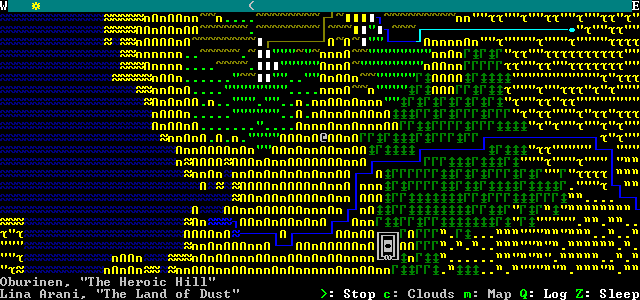
\includegraphics[width=6.25cm,height=4cm]{images/dwarffortress.png}
% 	\caption[]{A sample of the playable overworld in \emph{Dwarf Fortress}. Image sourced from: \url{http://www.bay12games.com}}
% 	\label{fig:fig1}
% 	\vspace{2ex}
% 	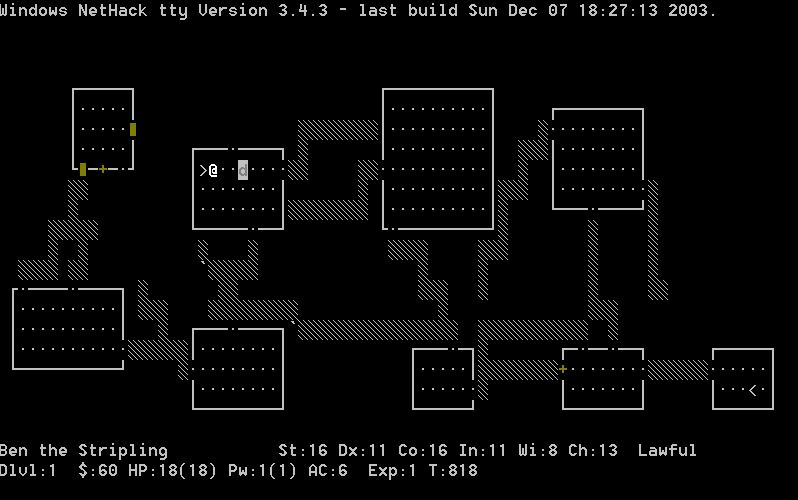
\includegraphics[width=6.25cm, height=4cm]{images/nethack3.png}
%   \caption[]{Typical generated dungeon structure in \emph{Nethack}.}
%   \label{fig:fig2}
% \end{figure}


\subsection{Deliverables}

The purpose of this work in summary was to investigate the various ways in which procedural content generation is used to generate game environments, and then design and build one or more variants based on the best of these approaches with the intent to create exciting and visually interesting in-game environments in a roguelike design space. The algorithm also intended to analyse created worlds to evaluate a measure of how interesting a world is, and only produce worlds that pass a set threshold to the player. Please note unfamiliar concepts in this section will be discussed in greater detail in section \ref{solutions}.\\

In order to achieve this, the project was split into basic, intermediate and advanced deliverables. The basic objective intended to produce a Java executable capable of handling user input, and output an ASCII grid output, providing a platform to display 2D ASCII environments for a player to explore indicative of the roguelike genre. The world generation algorithm was to be deterministic and include a 2D noise generator, providing the fundamental basis for procedural environment generation. The algorithm was then to provide a method of 2D noise smoothing, with the smoothing function able to produce explorable areas and structures for a player to explore. \\

We achieved the basic objective with an implementation in Java using the AsciiPanel library to produce a graphical user interface (GUI) to provide input and output to the player. A basic noise function of binary random output was created, and a smoothing function based on the \emph{Cellular Automata} ruleset was applied to form arbitrarily sized `caves' from the noise, explorable by a player.\\

The intermediate objectives were focussed on enhancing the in-game environment by implementing a more complex heightmap noise algorithm capable of producing more realistic in-game environments that exhibit contour behaviour, whereby the noise in one location is dependant on the surrounding elevation, mimicking the gradient nature of real-world environments. A further criteria was the that the generation algorithm was capable of operating efficiently, such that worlds could be evaluated based on a `variability' heuristic and then re-drawn instantaneously or even multiple times should a map not reach the thresholds set.\\


These intermediate objectives were achieved after researching various different noise algorithms. In the end, the fractal \emph{diamond-square} algorithm was adopted due its capability to produce contour based continuous heightmaps with low memory and CPU overheads, making it perfect for a roguelike game. This was then combined with a custom-made variant of the \emph{Cellular Automata} algorithm to smooth the noise, producing worlds that match the criteria to create more realistic worlds. Furthermore the efficient method of this noise generation and smoothing approach means that the variability coefficient- calculated by statistical analysis of the generated heightmap- can be used to evaluate worlds and regenerate worlds  on-the-fly that do not match up to the variability criteria set in order to make a world `interesting'. \\

The advanced criteria for this work was that worlds created should have `distinctive' features, and that worlds would be distinguishable on each playthrough to create a unique gaming experience that worked so well in \emph{Rogue} and subsequent derivatives. An extension to this includes the use of underlying mathematical functions, space-filling curves, that should exist within the structure of the heightmap to decrease the likelihood of encountering `dead ends' within game structures and increase player enjoyment.  Another aspect of the advanced criteria was that algorithm should also be able to identify connected regions of the map, with an understanding of how connected the produced environment is.\\

One of the advantages of procedural generation over traditional content production is the ability to create vastly different environments with minimal effort. We demonstrated this capability with the introduction of an overworld with a customisable probability function, allowing the developer to create a variety of different \emph{biomes} by adapting the heightmap transformation probabilities. Furthermore, we introduced the ability to feed in distinctive world features such as the \emph{Hilbert} space-filling curve to the noise generation algorithm, adding an underlying structure to the caves that are prevalent throughout the overworld. Finally, a breadth first \emph{flood-fill} search algorithm was used to identify connected regions of the map from the players position. \\


[This may well be too long]

\section{Related Work}

---- provide a narrative, not a list, so aim to structure this 
---- look at the lit survey? 
- CRITICAL ANALYSIS

- In this section it is important to note that work in this field comes from both academic sources but also work by amateur enthusiasts should not be ignored, but instead critically evaluated for its value. 
- draw from the very large active community 
- equally important 
- there exists many examples of different evaluation techniques 
- here we will discuss just some of the relevant examples from across big name games in the industry, 


- Talk about image generation of TerraGen - using midpoint displacement 

- Talk about other relevant examples of the algorithms i use

- Talk about perlin noise research and why i didnt use that- allude to the negatives of this approach/ scalability. talk about simplex noise also
	-- but implementation difficulty and runtime didn't match criteria for advanced objectives of tradeoff for worlds capabale of being produced quickly  


- Talk about the extended usage of these in minecraft and other things 

- Procedural generation as a subsection of other games eg something like borderlands but not
			-skin generation ?
			-population identification 
- Hilbert curve research? 

- Noise generation in amateur games - many references on this in my diss folder 

- Research into cellular automata? 

- Could talk about dwarf fortress/ other roguelikes 

- Canyon 3d work 
	- work by M carli et al on canyon creation using mean shift algorithm 
	- shows how you can bridge the gap between 2d and 3d, how 2d algorithms are relevant
	- explain that an implementation represented in 2d is still a 3-dimensional map just projected into 2d
	- k means 


\section{Solution} 
\label{solutions}

\subsection{Specification of Software}

The implementation of this work was developed and produced in Java (SE 1.8). There are a number of reasons why Java was well suited to this work. Java is a well established, high-level language preferred by thousands of amateur and professional game developers alike, and as such there are many previous implementations and libraries specific to roguelikes and procedural content generation from which this work was able to benefit from. By utilising copyright-free libraries and examples from previous roguelike enthusiasts, a quick prototype framework for the game was implemented and subsequently developed to form the foundation of the back-end of the game. This enabled the focus of the project to be on more important and interesting aspects of the generation algorithms. To this extent, many suitable libraries exist, and this work made particular use of the \emph{JFrame} and \emph{AsciiPanel} libraries, in addition to the \emph{Apache Commons Math} packages exising within the Java framework. \emph{JFrame} is a well known and established library enabling the use of a windowed frame for which the program is able to handle input and output, whereas \emph{AsciiPanel} is described as a `Java Console System Interface', popular among roguelikes and allowing for multi-colour ASCII text character output to the \emph{JFrame} environment. In addition to \emph{AsciiPanel}, the implementation made use of an open source framework developed by the creator of \emph{AsciiPanel}, providing access to the various functions that the \emph{AsciiPanel} library provides while allowing the project to focus on more complex aspects of the procedural generation algorithmic design \cite{trystan}. The capabilities of the resulting game engine allowed for an interactive window of a similar quality to that of estabilished roguelikes such as \emph{Nethack} and even \emph{Dwarf Fortress}\\

Java is also particularly useful due to its highly object-orientated nature. Since the design aspect of the game can be separated into many parts, it is helpful to be able to abstract and separate each process into different classes, allowing the main focus of the algorithmic side of the project to be apart from the engine handling input and output to the console. This makes development much easier, as well as improving bug fixing and code readability.\\

In addition, Java is known as a platform-neutral language \cite{java}, meaning the final implementation will be easily run on almost any platform (except mobile) without the need to recompile the source. This is very powerful and allowed for continued development and evaluation from a variety of computers during the project. \\

Finally, Java was chosen because of its familiarity. While the project may have benefited from features of other languages (such as the rapid prototyping and clear code style of Python), previous familiarity with Java enables a reduced implementation period in the system development life cycle, allowing more time to be spent on the design, planning and evaluation aspects of the cycle. 
\\

\subsection{Methodology}

The \emph{Agile} software development methodology was used in the project in order to meet its aims. This was selected because we felt that the project would benefit from achieving each functional target in individual rapid sprint cycles, which would then be able to be thoroughly tested for quality between cycles before the next implementation aspect was introduced. We also felt that this enabled a higher degree of freedom than other considered software development approaches (such as the \emph{Waterfall} approach), enabling the constant evaluation of the project at regular intervals.

\subsection{Noise and Smoothing Algorithms}

Noise algorithms form the foundation to most procedurally generated content and feature heavily in this work. The noise environment can then be modified by a variety of different approaches to form the basis of the content. There are a multitude of different noise algorithms [AS DEMONSTRATED IN THE RELATED WORK], however the basic objectives were achieved using discrete binary white noise, that is a 2-dimensional array of randomly assigned bits that are independent and theoretically identically distributed from each other \cite{stats}. 

\subsubsection{Cellular Automata}

The binary noise algorithm is simple and easy to implement, paving the foundation for a smoothing technique known as \emph{Cellular Automata}. This technique came about in the 1970s when British mathematician John Horton Conway devised his evolutionary \emph{Game of Life}, a game that transforms an initial state of `cells' into intricate and interesting patterns and designs by the use of 3 rules of state \cite{cellauto}:

\begin{itemize}
	\item Survivals: Every cell with two or three neighbouring cells of the same type survives for the next generation.
	\item Deaths: Each cell with four or more similar neighbours dies (is removed) from overpopulation. Every cell with one neighbour or none dies from isolation.
	\item Births: Each empty cell adjacent to exactly three neighbours--no more, no fewer--is a birth cell. A cell is placed on it at the next move.
\end{itemize}

This process is used upon the result of the binary white noise to `smooth' the landscape by turning areas that are mostly neighbouring walls into walls and areas neighbouring floors into floors, however we have adapted the ruleset in order for the algorithm to converge after a finite number of iterations- namely that cells do not `die' if they are surrounded by similar neighbours, and births are suppressed. The process is then repeated a number of times until the noise is sufficiently smoothed and the landscape converges towards a stable environment. 

\begin{figure}[ht]
  \centering
 	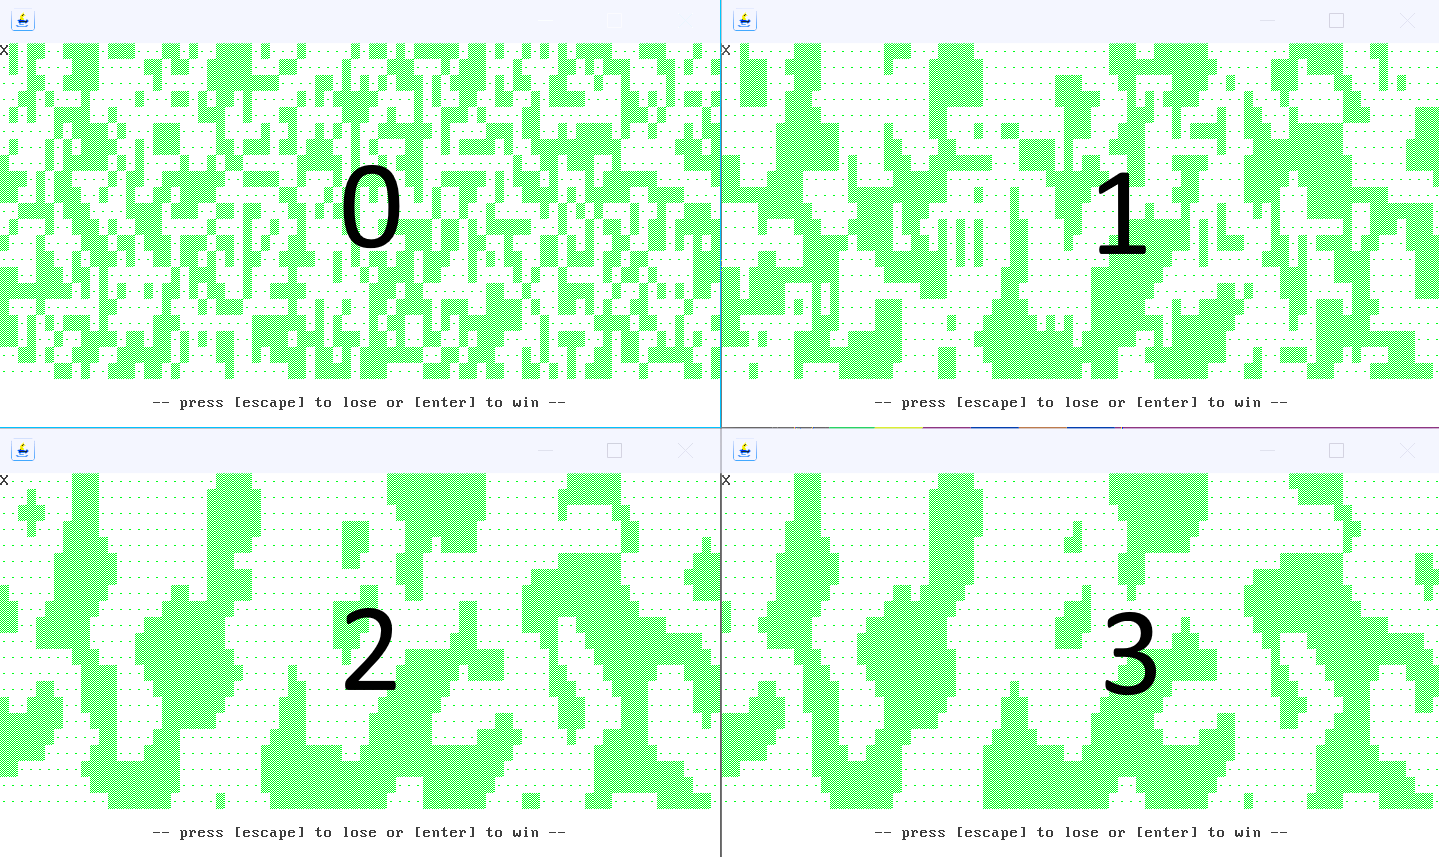
\includegraphics[scale=0.5]{images/cellauto.png}
	\caption[]{Cellular Automata cave smoothing. The numbers indicate the iterations of the algorithm, where the top-left image is before the smoothing process. Image self generated.}
	\label{fig:2}
\end{figure} 

It's clear to see from Figure \ref{fig:2} that this process very quickly converges to produce interesting, procedurally generated cave-like structures for a roguelike game setting, in addition to being computationally inexpensive (the generation is instantaneous even for very high levels of iterations (1000+) on a moderately powerful machine, and has time complexity O(wh) where w is the width and h is the height of a map \cite{cellularcomplexity}). \\

It is, however, limited in its usefulness by itself, as the results of the algorithm are inconsistent, occasionally producing uninteresting or unnatural worlds. Worse still, its particularly prone to what is known as `the isolated cave problem', whereby produced maps are often particularly `disconnected'- that is the player is often unable to advance to large regions of the cave. \\

This nature (seen in Figure \ref{fig:2}) is undesirable in order to fulfil the intermediate aims of the project, and a number of alternative approaches were considered to solve this problem.\\

One approach for example would be to generate many worlds and test for completeness, discarding the worlds that do not fit our criteria. Because of the instantaneous nature of this method of world population, we are able to create and evaluate many worlds very quickly, however the problem arises when we wish to expand our world size. A larger world boundary results in an increased statistical probability that the created world will be highly disjoint almost every time. An alternative approach would be to identify disjoint sections and post-process connect them up by removing wall segments. This does guarantee connectivity, but is also prone to making the world look unnatural, defeating the point of using the algorithm in the first place. One of the biggest advantages with \emph{Cellular Automata} however is that rules can be tweaked easily to modify the output to the developers preference, and this is exactly what amateur developers at \emph{RougeBasin} have done \cite{roguebasin}. By experimenting with the probabilities of birth and death rates, they are able to create connected caves that still maintain their natural look and feel.\\

This solution works well for smaller game environments, however even with the finest tweaking of parameters, its output is still unable to cope with larger maps of the nature this work aims to create. In this work, we come up with a different solution to the problem, owing to the use of both a completeness check using a breadth-first search and the introduction of space-filling curves, discussed in detail in section X and section Y respectively.  [REFERENCE]

\subsubsection{Diamond-Square Algorithm}

The above approach is a good starting point and has good potential for certain use cases, but even if it were possible to solve all of the aforementioned issues, it is fundamentally unable to create continuous heightmaps and struggles to create defining features; two aims of this project. With this in mind, we looked to more complex noise generation methods and while there are many available options, we selected the \emph{Diamond-Square} algorithm for this work. \\

THIS IS ALL BETTER OFF IN THE RELATED WORK SECTION----
The \emph{Diamond-Square} algorithm was initially proposed by Fournier, Fussell and Carpenter at the SIGGRAPH conference in 1982 and is an efficient way of generating fractal heightmaps in computer graphics \cite{FournierDSq}. It is particularly effective at modelling the contours of natural landscapes and is used by Planetside Software in their professional scenery generator program \emph{Terragen}\cite{claghorn}, whose outputs can be seen in popular movies such as \emph{Star Trek Nemesis} and \emph{The Golden Compass} \cite{planetside}. \\

It is important to point out however that the algorithm is not without its flaws and Gavin S. Miller notes in his 1986 paper \emph{The Definition and Rendering of Terrain Maps} that the algorithm is subject to `the creasing problem', whereby creases and slope discontinuities occur along the boundaries between fractals 
\cite{GMillerDiamondSq}. Having evaluated his argument however, we feel these negatives are outweighed by its fast evaluation time and impressive results, and are unlikely to become a problem in a roguelike setting. \\
---\\

The recursive algorithm starts with a square grid of dimension $n^2 + 1$ and giving random heights to the four corner values. The algorithm then recursively iterates over two steps, as shown in Fig \ref{fig:3} and summarised in brief below:

\begin{itemize}
	\item[]\emph{The Diamond Step:} Calculate the mean average of the 4 corners of a square and add a random perturbation to this value. The result is given to the value in the centre of the square, and produces 4 sided diamonds.
	\item[]\emph{The Square Step:} Calculate the mean average of the 4 points of each diamond and add a random perturbation to generate the value of the midpoint, producing more squares.
\end{itemize} 

The process is repeated recursively until every point in the grid is filled. However while this forms the foundation for the algorithm, we make a couple of modifications to the standard implementation to improve the results. The first is a measure to counteract the implementation issues that occur at the heightmap boundaries where there is no edge-side diamond value to use. While many applications simply ignore this condition at the edge and introduce edge artefacts, this work makes use of `edge wrapping', the concept of using the values at the opposing edge to complete the boundary cases. This is key to the prevention of edge artefacts, and even allows the algorithm to be used in an infinite basis, although that will not be explored in this work. 

The second is the variation parameter, $h$, which dictates how the world varies with respect to each iteration. Without a variable $h$, each iteration is free to vary from the last by whatever maximum height limit is set, however by reducing $h$ with each iteration, the smaller the square/diamond, the less the central midpoint value is allowed to deviate from its surroundings. Therefore, the variation function dictating how $h$ changes is key to how the algorithm reacts and behaves. These modifications are best seen in the psuedocode in Algorithm \ref{alg:1}.

\begin{algorithm}[H]
\SetAlgoLined
\KwData{arrayLength, seed, startingMaximum}
\KwResult{heightMap[][]}
Generate 2D array of type double = heightMap[][]\;
Initialise random number generator with seed = randGen()\;
Set corner values of heightmap with random perturbations\;
Initialise $h$ as startingMaximum/2\;
\While{heightMap is incomplete}{
\tcp{Diamond step}
Calculate square corner average = $avg$\;
Set midpoint = $avg$*h*randGen()\;
\tcp{Square step}
\If{boundary==true}{Get value from opposite side}
Calculate diamond corner average = $avg$\;
Set midpoint = $avg$*h*randGen()\;
$h$ = f($h$)\;
}

\caption{The Diamond-Square Algorithm }
\label{alg:1}
\end{algorithm}


\begin{figure}[ht]
  \centering
 	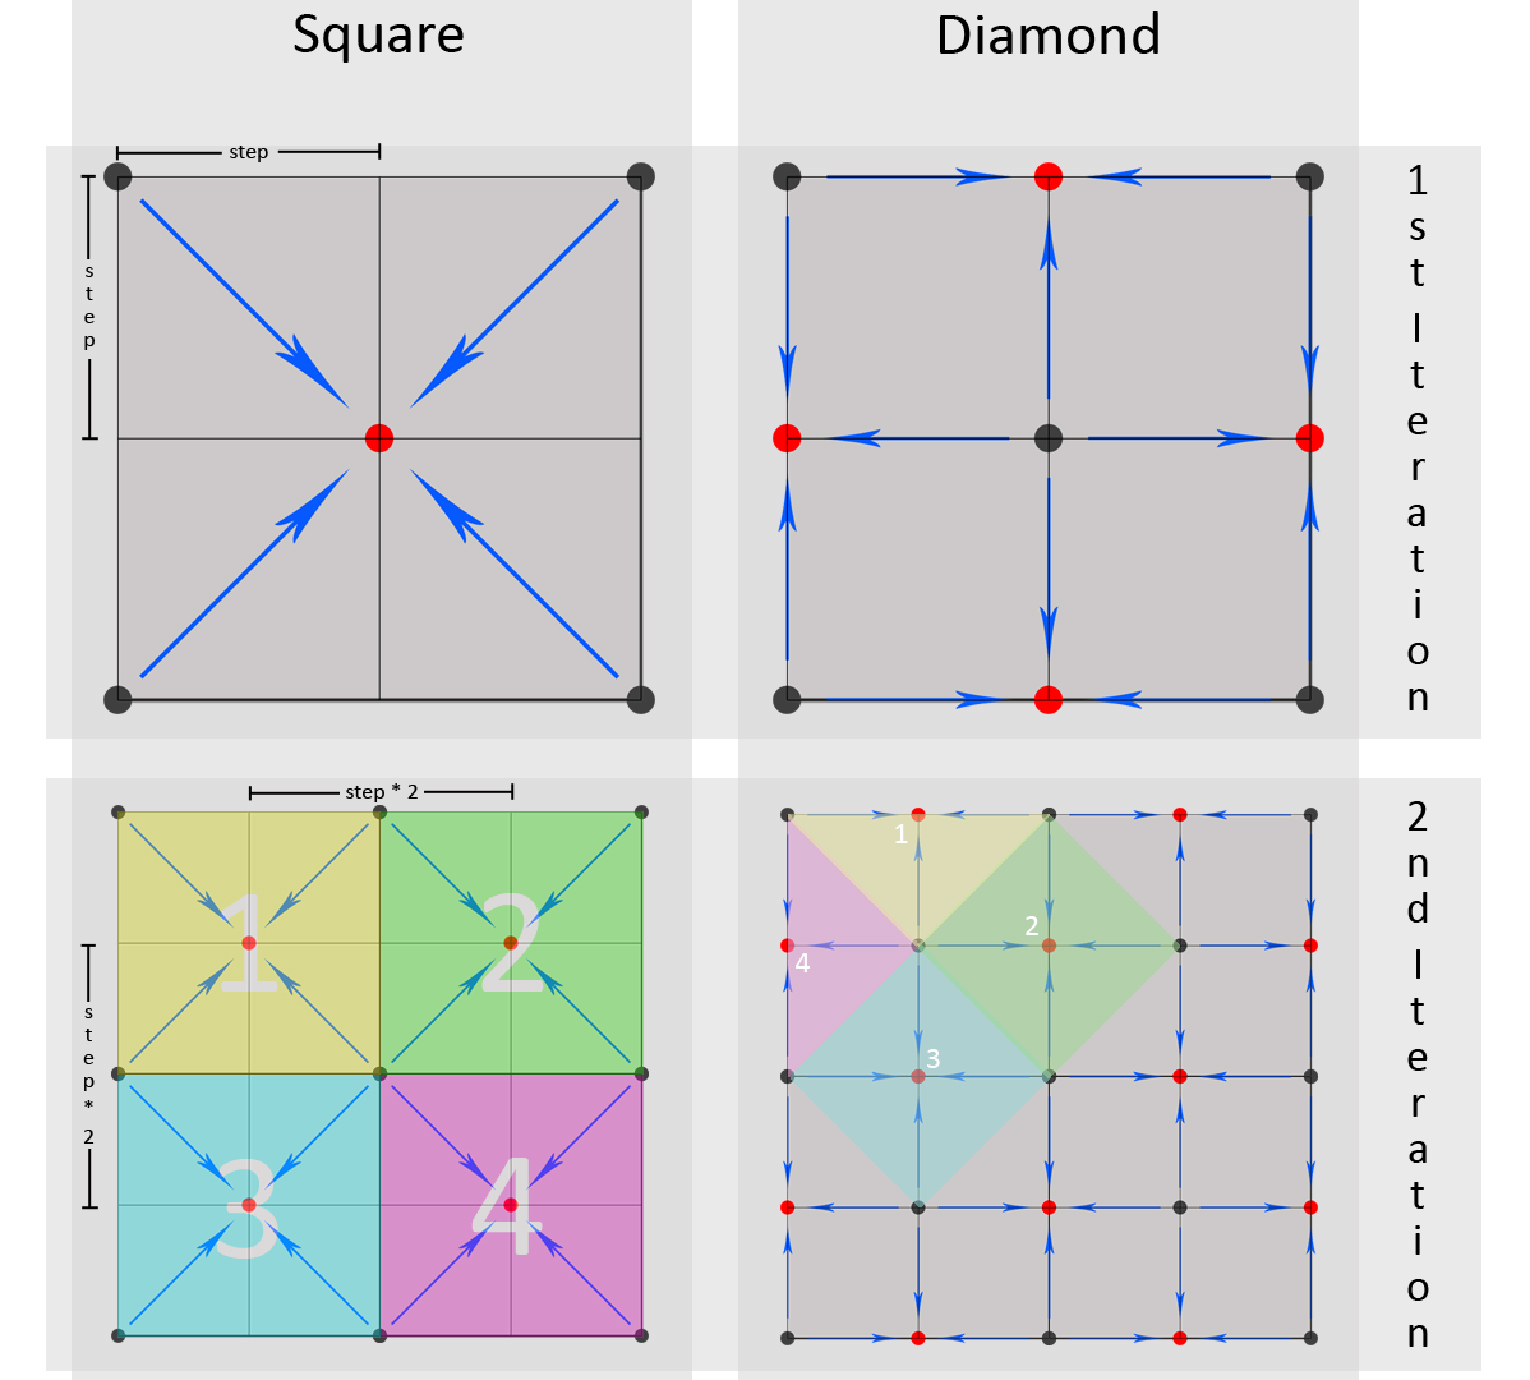
\includegraphics[width=0.4\linewidth]{images/diamondsquare.jpg}
	\caption[]{The process of the Diamond Square algorithm can be seen clearly here. Image taken from: \url{https://cmcbain.com/2014/07/31/procedural-terrain-generation-diamond-square-algorithm/}}
	\label{fig:3}
\end{figure} 


The resulting output of this produces a heightmap that can be used in conjunction with a set of tile transformation probabilities, allowing for the introduction of alternative tile types such as hills, forests, plains and mountains that occur at varying heights. Such depth adds considerable complexity to the game, expanding the number of ways the game can be played.\\ 

+ multiple biomes\\

\subsection{Space-Filling Curves}
+ ASCII feature read in \\

\subsection{Testing}

Unit testing?\\

Qualatitive testing \\

Bug testing- robust boundary stress testing by forcing boundary conditions \\


\subsection{Solution Pipeline}
(or something similar)\\
describes how each feature comes together \\

---\\
Mark Scheme \\
-Adequacy of the solution\\
-Specification and design\\
-Outline of implementation issues\\
-Description of tools used\\
	- and why\\
-Verification and validation\\
-Discussion of testing\\


\section{Results}

---Mark Scheme\\
-Evaluation method adopted? \\
-Clarity of the results - use python graphs?\\

Timing data\\

Use of parameters $h$, $v$ for variablility coefficient, $o$, the openness parameter\\

Parameters to be decided based on a range of values to be decided by user feedback -> which produces the most interesting results?\\



\section{Evaluation}

How suitable was my approach\\
- Agile caused problems \\
Appraisal of project organisation- what? \\

Strengths:\\
Produces excellent visual worlds most of the time\\
Ability to introduce arbitrary features inside caves from ASCII graphics \\
Very fast to generate worlds \\


Limitations:\\
Slow breadth first search\\
Only capable of doing square maps currently\\
Doesnt generate space filling curves by itself \\
Could report more statistical information to describe and shape worlds \\
Ability to add underlying ASCII only in caves \\




% - Talk about software enablers 
% 	- Java (SE 1.8)
% 	- Reiterate why java was chosen from design report 
% 	- talk about the prevalence of libraries 
% 	- abstraction 
% - platform neutral 
% - familiarity 

% 	look at the 3d canyon paper for a good example
% 	include psuedocode here for the diamond square algorithm and cellular automata 
% - Reinstate the aims 

-------------------

\section{Questions: } 

When to use \emph{Cellular Automata} or `Cellular Automata'
Psuedocode improvements? \\
References:\\
-too many urls?\\
-unnecessarily takes up lots of space currently \\
Linebreaks between paragraphs? \\
Image URL sources, shorten to goo.gl/asdfgh ?\\
Introduction- Shift some content to related work? \\
Related work:\\
-Roguelikes or wider context? \\
-Introduce perlin noise here? then talk about in evaluation why not used?\\

Concerned about lack of formal evaluative measures -> low marks for large sections





% \renewcommand{\bibfont}{\footnotesize}
\bibliography{bib}{} %Accesses bib.bib bibliography file

\bibliographystyle{unsrt} %Makes it so the numbers are ordered correctly

\end{document}